\documentclass{article}
\usepackage{amsmath}
\usepackage{hyperref}
\usepackage{graphicx}
\newcommand{\tabincell}[2]{\begin{tabular}{@{}#1@{}}#2\end{tabular}}

\begin{document}
\begin{titlepage}
\title{EE 239AS \\Special Topics in Signals and Systems\\Project 2\\Classification Analysis\\Winter 2016} 
\author{Liqiang YU, Kaiming WANG and Jun FENG\\
904592975, 504592374, 304588434} 
\date{02-21-2016}
\end{titlepage}

\maketitle
\newpage
\tableofcontents
\newpage
\section{Introduction}
In this report, we implemented some classification models to classify the textual data from the "20 Newsgroups" dataset, including support vector machine (SVM), naive Bayes classifier and logistic regression classifier. Before the classification,there were some data preprocessing steps, like changing the number in each subset to make them balanced, transforming the textual data into TF-IDF matrix, implementing the singular value decomposition to reduce the dimension of TF-IDF matrix. The task included binary classification and multiclass classification. The results were measured with the metrics including the average of precision, recall and accuracy. Moreover, in order to characterize the trade-off between true positive rate (TPR) and false positive rate (FPR), the receiver operating characteristic (ROC) curve was plotted.\\
\\
The report is organized as follows: In section 2, we plot the numbers of ducument in 8 required classes. In section 3, we first employ TF.IDF to get term features, then we use a `TF-IDF like' stategery to get the most significant terms in 4 required classes.in section \ref{sec:binary} we discussed the classification results with support vector machine, naive Bayes classifier and logistics regression classifier. We compared the results from two SVM models : hard margin SVM and soft margin SVM, computed the precision, recall, accuracy and confusion matrix, plotted the ROC curve from three models. In section \ref{sec:multi}, we implemented two strategies for multiclass classification : "one VS one" and "one VS rest" and repeated the above procedures to test the results.
\section{Dataset and Problem Statement}
From the API documentation, we know that the 20 newsgroups dataset comprises around 18000 newsgroups posts on 20 topics split in two subsets: one for training (or development) and the other one for testing (or for performance evaluation). The split between the train and test set is based upon a messages posted before and after a specific date. \\
\\
The first thing is to have a look at datesets, and the most direct way is to get the number of documents per classes.The figure is shown in figure \ref{fig:problema}. We can find that since the number of document from 8 classes -comp.graphics,comp.os.ms-windows.misc,comp.sys.ibm.pc.hardware,comp.sys.mac.hardware are almost the same. The total number of documents in Computer technology is \emph{2343} while number of documents in Recreational activity is \emph{2389}. So when analyzing these 8 classes, it is unnecessary to adjust the number of documents when conducting any analysis within only 8 classes. \\
\\
However, if we want to make the datasets more balanced, we should import the data randomly, and reduce the number of 20 classes to the lowest number of original classes. We can just get first intended number of documents per class.
\begin{figure}[htbp]
\centering
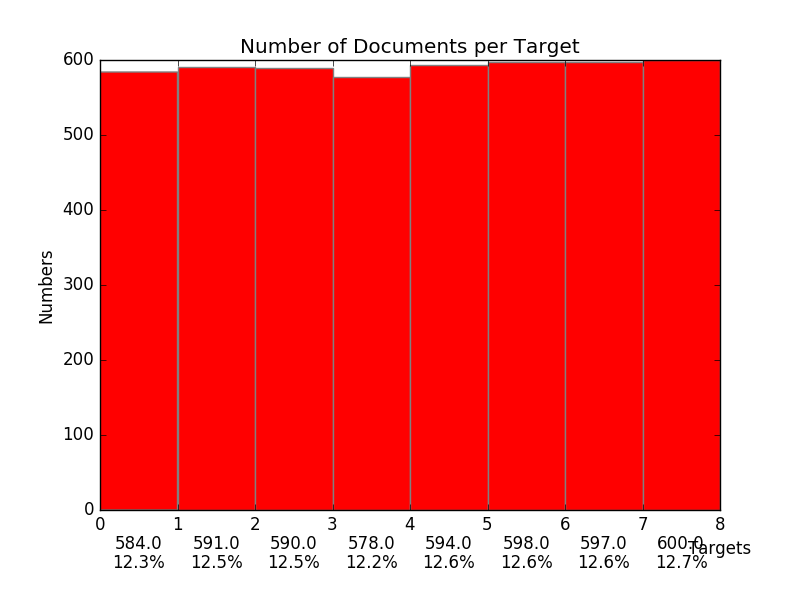
\includegraphics[width=.6\textwidth]{problema.png}
\caption{Numbers of Document per Target}
\label{fig:problema}
\end{figure}
\section{Modeling Text Data and Feature Extraction}
In this project, we will employ ``Big of Words'' assumption.The bag-of-words model is a simplifying representation used in natural language processing and information retrieval (IR). In this model, The text, or the document in our datasets, is represented as the bag (multiset) of its words, disregarding grammar and even word order. \\
\\
The bag-of-words model is commonly used in methods of document classification, where the (frequency of) occurrence of each word is used as a feature for training a classifier.However, before calculating the frequency of different terms, it is meaningful to remove different stems of verbs, stop words and punctuations.  By the way, we also remove special symbols and words containing numbers, since they are very rare.
\subsection{TFxIDF Vector Representations}
TF–IDF, which is the short for term frequency–inverse document frequency, is a numerical statistic that is intended to reflect how important a word is to a document in a collection or corpus.It is often used as a weighting factor in information retrieval and text mining. The tf-idf value increases proportionally to the number of times a word appears in the document, but is offset by the frequency of the word in the corpus, which helps to adjust for the fact that some words appear more frequently in general.\\
\\
We use TfidfVectorizer of sklearn to calculate the all \emph{11314} ducuments in 20 classes and finally we get \emph{54363} features.
\subsection{TFxICF and Significant Terms}
In this part, we would like to figure out whether a term is important to the class, so we can treat the whole set of documents in the same class as a ducument and calculate its TF.IDF, or so-called TF.ICF. However, we should pay attention that the defination of TF.ICF is one of common variation of IF.IDF, what is not used by the TfidfVectorizer of sklearn, we have to use CountVectorizer and try to achieve TF.ICF manually. Luckily, this procedure is quite easy. The result is in  Table \ref{10st}.
\begin{table}
\begin{center}
\caption{10 Most Significant Terms in 4 Classes }
\label{10st}
\begin{tabular}{|l||l|l|l|l|}
\hline
Rank & \tabincell{c}{comp.sys.ibm.\\pc.hardware} & \tabincell{c}{comp.sys.\\mac.hardware} & misc.forsale & soc.religion.christian \\
\hline
1& penev & powerbook & sabretoo & clh\\
2& balog & lcii & liefeld & liturgy\\
3& scsiha & iis & hobgoblin & kulikauska\\
4& husak & adb & uccxkvb & mmalt\\
5& laton & bmug & radley & copt\\
6& fasst & iivx & kou & caralv\\
7& buslog & iifx & keown & monophysit\\
8& korenek & jartsu & koutd & mussack\\
9& mbyet & firstclass & spiderm & sspx\\
10& dric & macus & mcfarlane & atterlep\\
\hline 	
\end{tabular}
\end{center}
\end{table}
\section{Binary Classification}\label{sec:binary}
In the binary classification problem, we chose eight classes and wanted to seperate them into two classes : Computer Technology and Recreational Activity. We assign the tag 0 to Computer Technology subclasses and tag 1 to Recreational Activity subclasses. The number of each subclass is almost the same so there is no need to balance them.
\subsection{Hard Margin SVM}
In the hard margin SVM, the objective function is
\begin{equation*}
min \frac{1}{2}\Vert W \Vert _2 ^2
\end{equation*}
And the constraints is
\begin{equation*}
y_i(W^T\overrightarrow{x_i}+b)\geq 1, i\in\lbrace 1, ..., n \rbrace
\end{equation*}
\\
In the program, we set C to 100000 to simulate the effect of hard margin. The average precision is 96.61\%, the average recall is 98.49\% and the accuracy is 97.49\%.The confusion table is shown in Table \ref{tb:confu}. The ROC curve  is shown in figure \ref{fig:roc}
\begin{table}
\begin{center}
\caption{The confusion matrix of hard margin SVM}
\label{tb:confu}
\begin{tabular}{|c|c|c|}
\hline
& Predicted Comp& Predicted Rect\\
\hline
Actual Comp&1505&55\\
\hline
Actual Rect&24&1566\\
\hline 	
\end{tabular}
\end{center}
\end{table}

\begin{figure}[htbp]
\centering
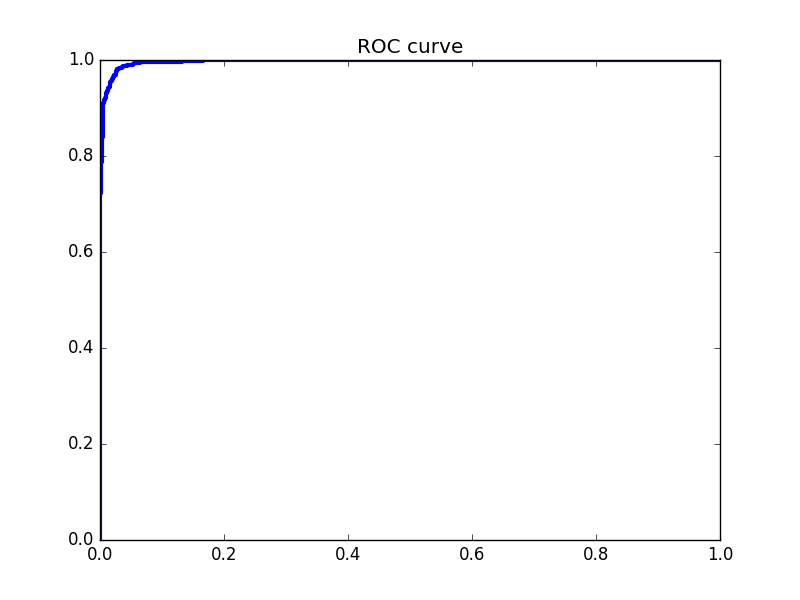
\includegraphics[width=.6\textwidth]{roc_hard.png}
\caption{The ROC curve of hard margin SVM}
\label{fig:roc}
\end{figure}
\subsection{Soft Margin SVM}
The problem of the hard margin model is that it may overfit the data, therefore it's better to use the soft margin SVM. In the soft margin model, we add error parameter in the objective function and the constraints. Thus the objective function is changed to the following:
\begin{equation*}
min \frac{1}{2}\Vert W \Vert _2 ^2 + \gamma\sum_{i=1}^{n}\xi _i
\end{equation*}
\\
Accordingly, the constraints are changed to the following:
\begin{equation*}
y_i(W^T\overrightarrow{x_i}+b)\geq 1-\xi _i,  \xi _i \geq0,  i\in\lbrace 1, ..., n \rbrace
\end{equation*}
\\
The $\gamma$ is the hyperparameter here and different $\gamma$ will affect the classification results. We implemented 5-fold cross validation to fit the model and choose the $\gamma$.  The best $\gamma$ we can get is 1000. The average precision is 96.61\%, the average recall is 97.96\% and the accuracy is 97.27\%. The confusion matrix is shown in Table \ref{tb:confu_soft}.The ROC curve is shown in figure \ref{fig:roc_soft}.
\begin{table}
\begin{center}
\caption{The confusion matrix of soft margin SVM with $\gamma$ = 100000}
\label{tb:confu_soft}
\begin{tabular}{|c|c|c|}
\hline
& Predicted Comp& Predicted Rect\\
\hline
Actual Comp&764&27\\
\hline
Actual Rect&16&769\\
\hline 	
\end{tabular}
\end{center}
\end{table}

\begin{figure}[htbp]
\centering
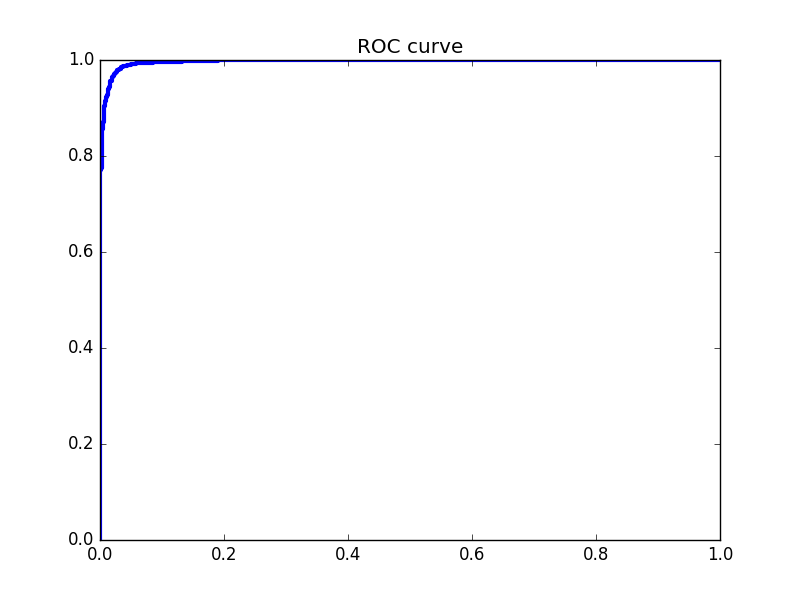
\includegraphics[width=.6\textwidth]{roc_soft.png}
\caption{The ROC curve for soft margin SVM}
\label{fig:roc_soft}
\end{figure}
\subsection{Naive Bayes Classifier}
Naive Bayes learning algotithm is based on Bayes' theorem and the word "naive" here means we adopt a "naive" assumption that the features are independent. Although the assumption looks over-simplified, the naive Bayes classifier works quite well in solving many practical problems. And it can be extremely fast.\\
\\
After using Latent Semantic Indexing, we get a matrix with negative values, which cannot be used to train a multinomial naive Bayes classifier. Thus, we first used our matrix to train a Gaussian naive Bayes classifier. And the predicted result shows the accuracy is 90.03\%, the precision is 91.54\% and the recall is 88.43\%. And the confusion matrix is shown in Table \ref{tb:confu_gnb}.\\
\begin{table}
\begin{center}
\caption{The confusion matrix of Gaussian naive Bayes classifier}
\label{tb:confu_gnb}
\begin{tabular}{|c|c|c|}
\hline
& Predicted Comp& Predicted Rect\\
\hline
Actual Comp&1430&130\\
\hline
Actual Rect&184&1406\\
\hline
\end{tabular}
\end{center}
\end{table}
\\
The ROC of this classifier is shown as Figure \ref{fig:roc_gnb} and the area under the curve(AUC) is 0.9633.\\
\begin{figure}[htbp]
\centering
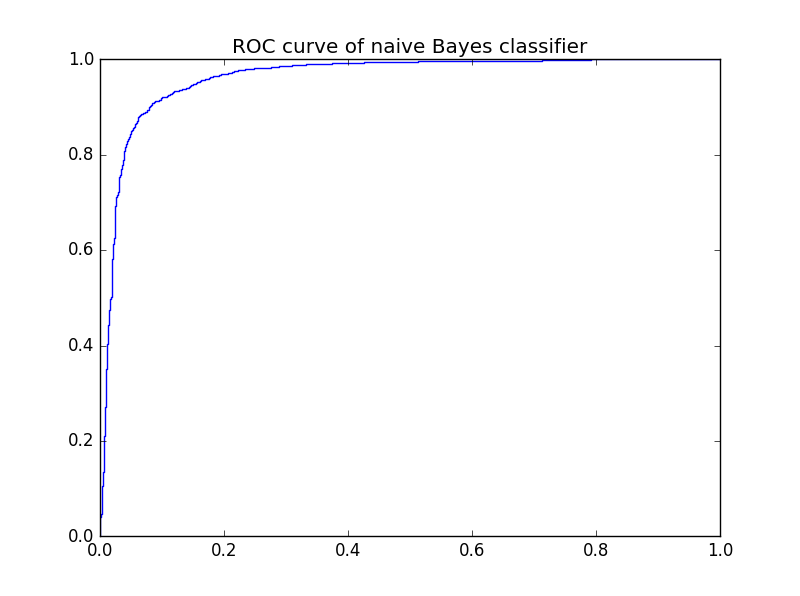
\includegraphics[width=.6\textwidth]{g_gaus_naive_bayes_roc.png}
\caption{The ROC curve of Gaussian naive Bayes classifier}
\label{fig:roc_gnb}
\end{figure}
\\
Then, we try to implement a Bernoulli naive Bayes classifier instead, which is also suitable for text classification and may be even better than the multinomial one. Actually, the main difference between these two is that the Bernoulli classifier penalizes the non-occurrence of a feature explicitly. However, we should notice that the Bernoulli classifier is only suitable for binary-valued features, so here we must first implement binarization to our features before using it to train our classifier.\\
\\
The prediction tells that the accuracy is 90.96\%, the precision is 90.81\% and the recall is 91.32\%. The confusion matrix is shown in Table \ref{tb:confu_bnb}.\\
\begin{table}
\begin{center}
\caption{The confusion matrix of Bernoulli naive Bayes classifier}
\label{tb:confu_bnb}
\begin{tabular}{|c|c|c|}
\hline
& Predicted Comp& Predicted Rect\\
\hline
Actual Comp&1413&147\\
\hline
Actual Rect&138&1452\\
\hline
\end{tabular}
\end{center}
\end{table}
\\
The ROC curve is plot as Figure \ref{fig:roc_bnb} and the AUC is 0.9633.\\
\begin{figure}[htbp]
\centering
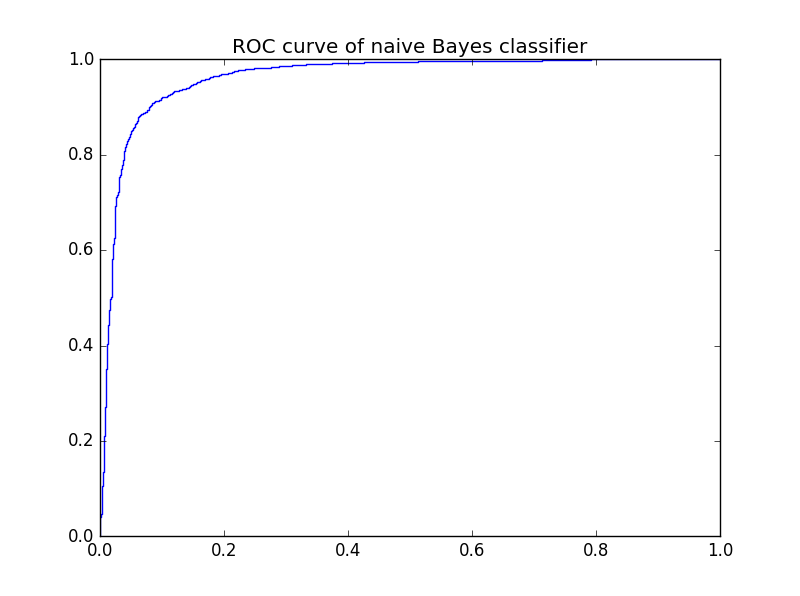
\includegraphics[width=.6\textwidth]{g_naive_bayes_roc.png}
\caption{The ROC of Gaussian naive Bayes classifier}
\label{fig:roc_bnb}
\end{figure}
\\
From this results, we may learn that the performance of this two kinds of classifier is very similar and both can achieve an accuracy about 90\%.\\

\subsection{Logistic Regression Classifier}
The last algorithm we will applied for binary classifier is the logistic regression algorithm, which is a linear model for classification. And there is two alternatives, L1 or L2 regularization, of penalization function for the optimization problem behind this algorithm. In our experiment, we implement both of them and try to compare their outcomes.\\
\\
Under L1 regularization, the predicted result shows the accuracy is 96.73\%, the precision is 95.98\% and the recall is 97.61\%. The confusion matrix is shown as Table \ref{tb:confu_lr1}.\\
\begin{table}
\begin{center}
\caption{The confusion matrix of L1 logistic regression classifier}
\label{tb:confu_lr1}
\begin{tabular}{|c|c|c|}
\hline
& Predicted Comp& Predicted Rect\\
\hline
Actual Comp&1495&65\\
\hline
Actual Rect&38&1552\\
\hline
\end{tabular}
\end{center}
\end{table}
\\
The ROC curve is shown in Figure \ref{fig:roc_lr1} and its AUC is 0.9956.\\
\begin{figure}[htbp]
\centering
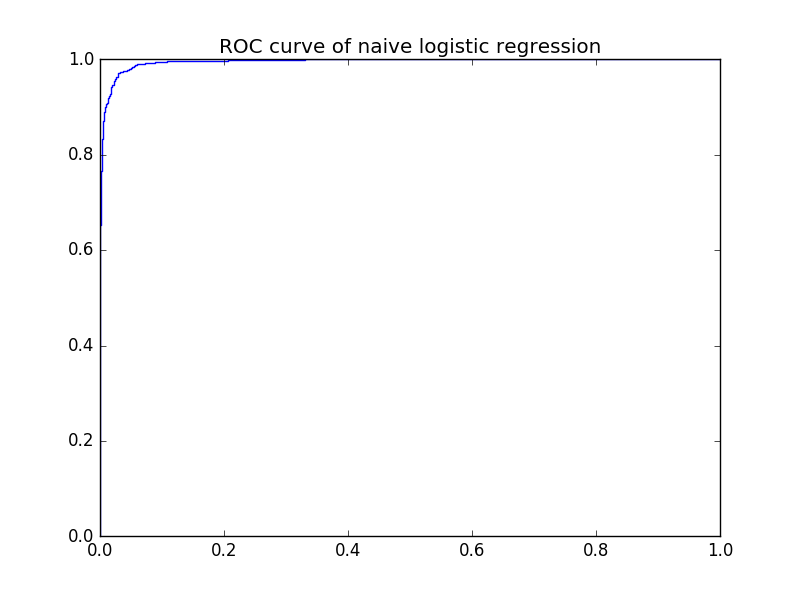
\includegraphics[width=.6\textwidth]{h_logistic_regression_l1_roc.png}
\caption{The ROC of L1 logistic regression classifier}
\label{fig:roc_lr1}
\end{figure}
\\
If we use L2 regularization, the accuracy of predictions is 96.54\%, the precision is 95.34\% and the recall is 97.92\%. The confusion matrix is shown as Table \ref{tb:confu_lr2}.\\
\begin{table}
\begin{center}
\caption{The confusion matrix of L2 logistic regression classifier}
\label{tb:confu_lr2}
\begin{tabular}{|c|c|c|}
\hline
& Predicted Comp& Predicted Rect\\
\hline
Actual Comp&1484&76\\
\hline
Actual Rect&33&1557\\
\hline
\end{tabular}
\end{center}
\end{table}
\\
The ROC curve is shown in Figure \ref{fig:roc_lr2} and its AUC is 0.9950.\\
\begin{figure}[htbp]
\centering
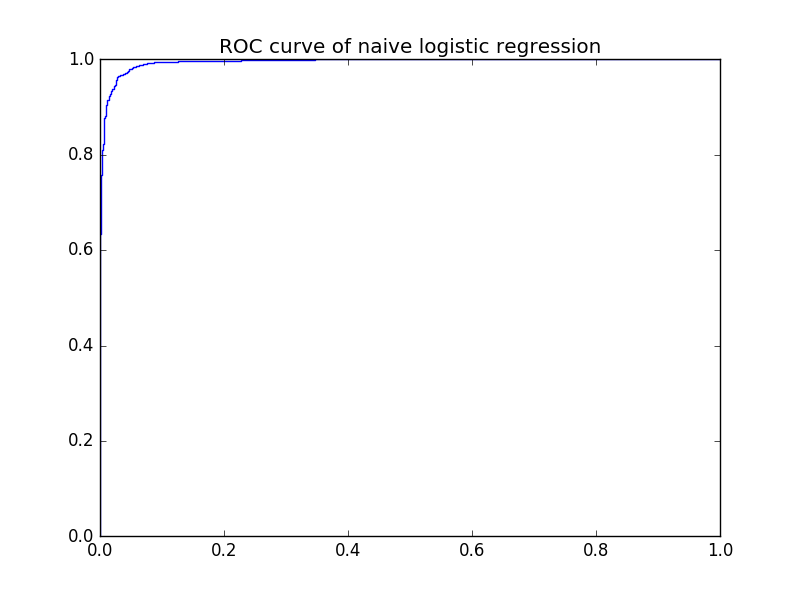
\includegraphics[width=.6\textwidth]{h_logistic_regression_l2_roc.png}
\caption{The ROC of L2 logistic regression classifier}
\label{fig:roc_lr2}
\end{figure}
\\
From these outcomes, we may suppose that when trained with the data after process of LSI, the form of regularization does not affect the performance of the logistic regression classifier a lot.\\
\\
The ROC curves of all the classifiers all plot in Figure \ref{fig:roc}.\\
\begin{figure}[htbp]
\centering
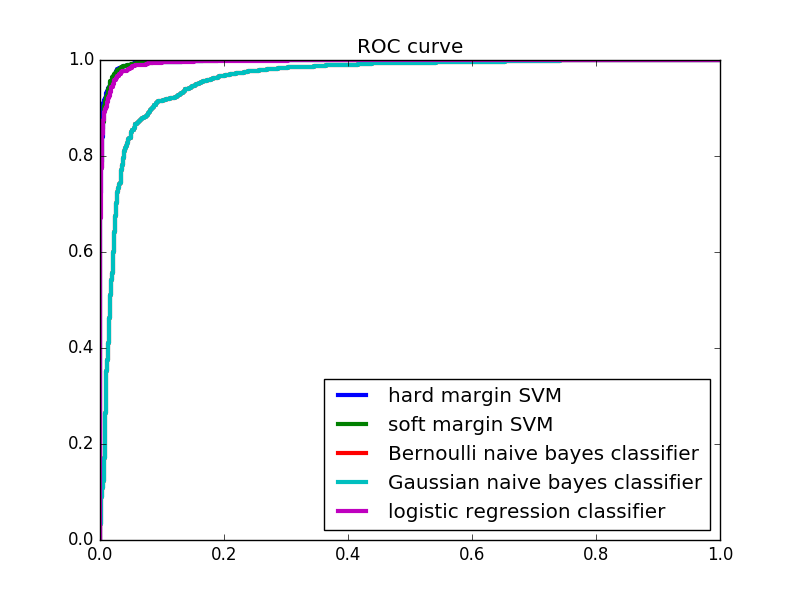
\includegraphics[width=.6\textwidth]{roc.png}
\caption{The ROC curve for all classifiers}
\label{fig:roc}
\end{figure}

\section{Multiclass Classification}\label{sec:multi}
From now on, we will try to solve the multiclass classification with some of the algorithm we have used before.\\
\\
Before classifying, we first discuss about the unbalancing between the 4 target classes. After counting, the number of files in each class is shown as Table \ref{tb:filenum}, from which we know that all the 4 classes have about 390 files. Thus, it is already well-balanced.\\
\begin{table}
\begin{center}
\caption{The number of files of each class}
\label{tb:filenum}
\begin{tabular}{|c|c|}
\hline
Class name&Number of files\\
\hline
comp.sys.ibm.pc.hardware&392\\
comp.sys.mac.hardware&385\\
misc.forsale&390\\
soc.religion.christian&398\\
\hline
\end{tabular}
\end{center}
\end{table}

\subsection{Naive Bayes Classifier}
The naive Bayes classifier perform the multiclass classification inherently. It simply finds out the class with the maximun likelihood given the data. And in our experiments, we still implement both Gaussian and Bernoulli naive Bayes classifiers exactly the same as in binary classification.\\
\\
The results of Gaussian classifier is that the accuracy is 67.09\%(notice that the statistics we represent here is the mean among all the four classes, if needed we can get it of each class from the confusion table), the precision is 70.22\% and the recall is 67.09\%.\\
\\
The confusion matrix is shown in Table \ref{tb:confu_mul_gnb}.\\
\begin{table}
\begin{center}
\caption{The confusion matrix of Gaussian naive Bayes classifier}
\label{tb:confu_mul_gnb}
\begin{tabular}{|c|c|c|c|c|}
\hline
Predicted&pc.hardware&mac.hardware&forsale&christian\\
\hline
Actual pc.hardware&244&36&112&0\\
\hline
Actual mac.hardware&98&142&144&1\\
\hline
Actual forsale&41&36&313&0\\
\hline
Actual christian&4&0&43&351\\
\hline
\end{tabular}
\end{center}
\end{table}
\\
From this results, we know that the performance of Gaussian classifier is much worse than binary case. It only achieves a 70\% accuracy. We may notice that most of the errors occur between the first two classes, from the name of which we may suggest that the content of them are quite similar. As a result, this simple classifier can not well distinguish them.\\
\\
To solve this problem, we try to implement a Bernoulli naive Bayes classifier. The result of this is we get an accuracy of 83.07\%, a precision of 83.20\% and a recall of 83.07\%. And the confusion matrix is shown in Table \ref{tb:confu_mul_bnb}.\\
\begin{table}
\begin{center}
\caption{The confusion matrix of Bernoulli naive Bayes classifier}
\label{tb:confu_mul_bnb}
\begin{tabular}{|c|c|c|c|c|}
\hline
Predicted&pc.hardware&mac.hardware&forsale&christian\\
\hline
Actual pc.hardware&296&69&25&2\\
\hline
Actual mac.hardware&65&296&21&3\\
\hline
Actual forsale&42&28&314&6\\
\hline
Actual christian&2&1&1&394\\
\hline
\end{tabular}
\end{center}
\end{table}
\\
The statistics and the confusion matrix show that,under this case, the Bernoulli's one is much better than the Gaussian's. Although the errors still happen most frequently between the first two classes, the total number of them has decreased. We suggest this is mainly because the feature binarization, after which we can distinguish the ibm pc and the mac.

\subsection{One VS One SVM}
To implement SVM for multiclass classification, one way is to create a set of one-to-one SVMs between each pair of target classes, each of which vote for one of the two classes for a given data. And the class with highest votes is picked as the result.\\
\\
In our program, we implement soft margin SVMs and set the $\gamma$ of them to 100. And the statistics of the predictions is that the accuracy is 88.17\%, the precision is 88.23\% and the recall is 88.18\%.\\
\\
The confusion matrix is shown in Table \ref{tb:confu_mul_svm_ovo}
\begin{table}
\begin{center}
\caption{The confusion matrix of 1 VS 1 SVM classifier}
\label{tb:confu_mul_svm_ovo}
\begin{tabular}{|c|c|c|c|c|}
\hline
Predicted&pc.hardware&mac.hardware&forsale&christian\\
\hline
Actual pc.hardware&318&50&24&0\\
\hline
Actual mac.hardware&36&323&26&0\\
\hline
Actual forsale&26&16&348&0\\
\hline
Actual christian&4&1&2&391\\
\hline
\end{tabular}
\end{center}
\end{table}

\subsection{One VS Rest SVM}
Another way to implement SVM for multiclass classification is to create a set of one versus rest SVMs for every classes. Since here we only need n classifiers for n classes, the efficiency is achieved. Besides, since each class is represented by a classifier, it is convenient for us to gain knowledge of the classes.\\
\\
In our program, we implement soft margin SVMs and set the $\gamma$ of them to 100. And the statistics of the predictions is that the accuracy is 88.63\%, the precision is 88.65\% and the recall is 88.63\%.\\
\\
The confusion matrix is shown in Table \ref{tb:confu_mul_svm_ovr}
\begin{table}
\begin{center}
\caption{The confusion matrix of 1 VS rest SVM classifier}
\label{tb:confu_mul_svm_ovr}
\begin{tabular}{|c|c|c|c|c|}
\hline
Predicted&pc.hardware&mac.hardware&forsale&christian\\
\hline
Actual pc.hardware&318&45&27&2\\
\hline
Actual mac.hardware&32&326&26&1\\
\hline
Actual forsale&19&15&354&2\\
\hline
Actual christian&5&1&3&389\\
\hline
\end{tabular}
\end{center}
\end{table}
\\
First thing we learn from the result of these two kinds of SVM classifiers is that their outperform the naive Bayes classifiers and achieve an accuracy of near 90\%. After a more a closer observation, we can say that the first two classes are very similar to each other while the last class is most different from all the others.

\section{Conclusion}
In this project, we aimed to finish some classification tasks with the textual data provided by the "20 Newsgroup" dataset. We classified 8 subclasses into 2 classes with the hard margin SVM, soft margin SVM, naive Bayes classifier and logistics regression classifier. The comprehensive results is shown in the Table \ref{tb:binaryresults}. As for the multiclass classification, the comprehensive results is shown in Table \ref{tb:multiresults}.
\begin{table}
\begin{center}
\caption{The comprehensive results of binary classification}
\label{tb:binaryresults}
\begin{tabular}{|c|c|c|c|}
\hline
& Accuracy& Precision& Recall\\
\hline
hard margin SVM& 97.49\%&96.61\% &98.49\% \\
\hline
soft margin SVM& 97.27\%&96.61\% &97.96\% \\
\hline 	
Bayes&90.95\% &90.81\% & 91.32\%\\
\hline
Logistic Regression& 96.73\%&95.98\% &97.61\%\\
\hline
\end{tabular}
\end{center}
\end{table}

\begin{table}
\begin{center}
\caption{The comprehensive results of multiclass classification}
\label{tb:multiresults}
\begin{tabular}{|c|c|c|c|}
\hline
& Accuracy& Precision& Recall\\
\hline
1-1 SVM& 88.18\%&88.23\% &88.18\% \\
\hline
1-rest SVM& 88.63\%&88.65\%&88.63\%\\
\hline
Gaussian naive Bayes& 67.09\%& 70.22\%& 67.09\%\\
\hline
Bernoulli naive Bayes& 83.07\%&83.20\%& 83.07\%\\
\hline
\end{tabular}
\end{center}
\end{table}
\end{document}